\documentclass[11pt]{article}
%\def\hidesolutions{}
%%%%%%%%%%% SET MARGINS
\setlength{\textheight}{20cm}
\setlength{\topmargin}{-0.5cm}
\setlength{\oddsidemargin}{+0cm}
\setlength{\textwidth}{16.3cm}
%\setlength{\parskip}{6pt}
\setlength{\parindent}{0pt}

%%%%%%%%%%% PACKAGES
\usepackage{amsmath}
\usepackage{amssymb}
\usepackage{amsfonts}
%\usepackage{a4wide}
\usepackage{graphicx}
\usepackage{color}
\usepackage[normalem]{ulem}
\usepackage{enumitem}
\usepackage{capt-of}
\usepackage{float}
\usepackage{amsmath}
\usepackage{listings}
\definecolor{mygreen}{RGB}{28,172,0} % color values Red, Green, Blue
\definecolor{mylilas}{RGB}{170,55,241}
\usepackage{empheq}
\usepackage[ruled]{algorithm2e}
\usepackage{mathrsfs}
\usepackage{datetime}
\usepackage{subcaption}

% TODO: combine the two package lists and reduce redundancies 
\usepackage{mathtools}
\usepackage{nicefrac}
\usepackage{hyperref}
\usepackage{url}
\usepackage{amsmath,amssymb,amsfonts}
\usepackage{a4wide}
\usepackage{graphicx}
\usepackage{color}
\usepackage[normalem]{ulem}
\usepackage{capt-of}
\usepackage{float}
\usepackage[ruled]{algorithm2e}
\usepackage{amsmath,amssymb,amsfonts}
\usepackage{a4wide}
\usepackage{graphicx}
\usepackage{color}
\usepackage[normalem]{ulem}
\usepackage{capt-of}
\usepackage{float}
\usepackage[ruled]{algorithm2e}
\usepackage{mathrsfs}







\newcommand{\Lc}[2]{{\color{blue} \sout{#1} } \textcolor{red}{#2}}
\newcommand{\La}[1]{\textcolor{red}{#1}}
\newcommand{\lh}{\mathscr{L}_h}
\newcommand{\cl}{\mathscr{L}}
\newcommand{\cf}{\mathscr{F}}
\newcommand{\dx}{dx}
% \newcommand{\d}{d}
\newcommand{\ltn}{\mathscr{l}^2}
\newcommand{\bbR}{\mathbb{R}}
\newcommand{\Rset}{\mathbb{R}}
\newcommand{\Nset}{\mathbb{N}}
\newcommand{\scL}{\mathcal{L}}
\newcommand{\xx}{\mathbf{x}}
\newcommand{\norm}[1]{\|{#1}\|}
\newcommand{\yy}{\mathbf{y}}
\newcommand{\at}[1]{\big|_{#1}}
\renewcommand{\div}{\mathrm{div}}
\newcommand{\divergence}{\mathrm{div}}
\newcommand{\cp}[1]{\textcolor{blue}{#1}}

\newcommand{\FF}{\texttt{FreeFem++ }}
\newcommand{\FFns}{\texttt{FreeFem++}}
\newcommand{\FFfull}{\texttt{FreeFem++-x11}}
\newcommand{\cmd}[1]{ \medskip \noindent \texttt{#1} \medskip}
\newcommand{\incmd}[1]{\texttt{#1}}
\newcommand{\shrinkitems}{\addtolength{\itemsep}{-0.5\baselineskip}}
\newcommand{\mtt}[1]{\mathtt{#1}}
\newcommand{\ML}{\texttt{Matlab }}

\newcommand{\bb}{\mathbf{b}}
\newcommand{\nn}{\mathbf{n}}
\newcommand{\vecA}{\vec{A}}
\newcommand{\vecB}{\vec{B}}


\newcommand{\frakF}{\mathfrak{F}}


\newcommand{\mesh}{\mathcal{T}_h}
\newcommand{\refel}{\widehat{K}}
\newcommand{\ver}{\mathbf{a}}
\newcommand{\refver}{\widehat{\mathbf{a}}}
\newcommand{\grad}{\nabla}
\newcommand{\refgrad}{\widehat{\nabla}}
\newcommand{\refu}{\widehat{u}}
\newcommand{\refbasis}{\widehat{\varphi}}
\newcommand{\refxx}{\widehat{\xx}}
\newcommand{\refx}{\widehat{x}}
\newcommand{\refy}{\widehat{y}}
\newcommand{\refrho}{\widehat{\rho}}
\newcommand{\refh}{\widehat{h}}

\makeatletter
\newcommand\suchthat{%
 \@ifstar
  {\mathrel{}\middle|\mathrel{}}
  {\mid}%
}
\makeatother





% For typesetting Python code
\newcommand{\matlab}{{\sc Matlab}\xspace}
\usepackage{listings}
\lstloadlanguages{Python}
\lstloadlanguages{csh}%
\definecolor{MyDarkGreen}{rgb}{0.0,0.4,0.0}
\definecolor{purple}{rgb}{0.58,0,0.82}
\lstset{language=Python,                    % Use Python
	%frame=single,                          % Single frame around code
	basicstyle=\ttfamily\footnotesize\color{black},
	keywordstyle=[1]\color{blue}\bf,        % Python functions bold and blue
	keywordstyle=[2]\color{purple},         % Python function arguments purple
	keywordstyle=[3]\color{red}\underbar,   % User functions underlined and blue
	commentstyle=\usefont{T1}{pcr}{m}{sl}\color{MyDarkGreen}\small,
	stringstyle=\color{purple},
	showstringspaces=false,                 % Don't put marks in string spaces
	tabsize=3,                              % 5 spaces per tab
	morekeywords={xlim,ylim,var,alpha,factorial,poissrnd,normpdf,normcdf},
	morecomment=[l][\color{blue}]{...},
	breaklines=true,
	breakatwhitespace=true,
	emptylines=1,
	mathescape=true,
	xleftmargin=0ex,
	emphstyle=\bfseries\color{red}
}





%%%%%%%%%%% MACROS NAMES
\newcommand{\lecturername}{Martin Licht}
% \newcommand{\assistantnamea}{Jochen Hinz}
% \newcommand{\assistantnameb}{Ivan Bioli}
\newcommand{\semestername}{Winter Semester 2024}
\newcommand{\lecturename}{Analysis III - 203(d)}
\DeclarePairedDelimiter\floor{\lfloor}{\rfloor}

%%%%%%%%%%% HEADER
\newdateformat{yeardate}{\THEYEAR}
\newcommand{\exsheet}[3] % input is the number of the session and the day TODO What's that
{\clearpage

	\begin{center}
		{\Large \textbf{\lecturename}}\\[2ex]
		\semestername
	\end{center}

	% \vspace{2ex}
	% \lecturername

	\vspace{2ex}
	{\Large Session #1: #3\,#2, \yeardate\today}
	%\hfill
	%{\Large EPF Lausanne}

	\hrulefill
}





\usepackage{comment}

\newtheorem{exercise}{Exercise}
\newtheorem{solutionenv}{Solution}

\newboolean{hide_solution}
\ifx\hidesolutions\undefined
\newenvironment{solution}{\begin{solutionenv}}{\end{solutionenv}}
\setboolean{hide_solution}{false}
\else
\excludecomment{solution}
\setboolean{hide_solution}{true}
\fi

\newcommand{\ifnotsolution}[1]{\ifthenelse{\boolean{hide_solution}}{#1}{}}
\newcommand{\ifsolution}[1]{\ifthenelse{\boolean{hide_solution}}{}{#1}}


\usepackage{tikz}
\usepackage{pgfplots}





\allowdisplaybreaks

\begin{document}
\exsheet{8}{7}{November} % parameters are the number of the session and the day















\begin{exercise} % 5
    Consider the surface 
    \begin{align*}
        S := \left\{ \vec x \in \bbR^{3} \suchthat* \|x\| = 1, x_3 > 0 \right\}
    \end{align*}
    \begin{itemize}
    \item Find a parameterization of $S$ and find the unit normal corresponding to that parameterization.
    \item Find a parameterization of $C = \partial S$.
    \item Verify Stokes theorem with the vector field 
     \begin{align*}
        \vec F(x_1,x_2,x_3) = ( -x_2, x_1, x_3 ).
     \end{align*}   
    \end{itemize}
\end{exercise}
\begin{solution}     
    \begin{itemize}
    \item 
    $$
        \Phi: \Omega:= [0,2\pi)\times[0,\frac{\pi}{2}) \mapsto S: (\theta,\phi)\mapsto (\cos\theta\sin\phi,\sin\theta\sin\phi,\cos\phi) 
    $$
    $$
        \vec{n} = \frac{\partial_{\theta}\Phi\times \partial_{\phi}\Phi}{||\partial_{\theta}\Phi\times \partial_{\phi}\Phi||} = \begin{pmatrix}\cos\theta\sin\phi \\ \sin\theta\sin\phi\\ \cos\phi\end{pmatrix}
    $$

    \item 
    We first parameterize the boundary of the parameter space $\Omega$ 
    $$
        \gamma:[0,2\pi) \mapsto \partial \Omega : \theta \mapsto(\theta, \frac{\pi}{2}),
    $$
	which gives us the parameterization of the boundary as follows:
    $$
        \Phi\circ \gamma:[0,2\pi) \mapsto \partial C : \theta \mapsto(\cos\theta,\sin\theta,0).
    $$

    \item 
    We have to show that:
    $$
    \iint_S \nabla \times \vec{F} d\sigma = \oint_C \vec{F} d\ell
    $$
    \begin{align*}
        \iint_S \nabla \times \vec{F} d\sigma &= \iint_S \nabla \times \vec{F}\cdot \vec{n}||\partial_{\theta}\Phi\times \partial_{\phi}\Phi|| d\sigma\\
        &= \iint_S \begin{pmatrix} 0\\ 0\\ 2 \end{pmatrix}\cdot \begin{pmatrix}\cos\theta\sin\phi \\ \sin\theta\sin\phi\\ \cos\phi\end{pmatrix}\sin\phi d\sigma\\
        &= \int_0^{2\pi}\int_0^{\frac{\pi}{2}} 2\cos\phi\sin\phi d\phi d\theta\\
        &= \int_0^{2\pi}\int_0^{\frac{\pi}{2}} \sin2\phi d\phi d\theta\\
        &= 2\pi \left[ -\frac{1}{2}\cos2\phi \right]_0^{\frac{\pi}{2}} = 2\pi\\
    \end{align*}   
    \begin{align*}
        \oint_C \vec{F} d\ell &= \int_0^{2\pi} \vec{F}(\Phi\circ \gamma)\cdot \frac{d(\Phi\circ \gamma)}{d\theta}  d \theta\\
        &= \int_0^{2\pi} \begin{pmatrix} -\sin\theta\\ \cos\theta\\ 0 \end{pmatrix}\cdot \begin{pmatrix}-\sin\theta \\ \cos\phi \\ 0\end{pmatrix} d \theta\\
        &= \int_0^{2\pi} 1 d \theta = 2\pi\\
    \end{align*}   
    \end{itemize}
\end{solution}















\begin{exercise} % 4
    Let $S$ be the surface with parameterization $\Phi : \Omega \to S$ as follows:
    \begin{align}
     S := \left\{ \vec x \in \bbR^3 \suchthat* x_1^2 + x_2^2 = 1, \; -1 < x_3 < 1 \right\},
    \end{align}
    Suppose we have a vector field 
    \begin{align}
        \vec F(x_1,x_2,x_3) := (x_2 x_3, -x_1 x_3, 0 ).
    \end{align}
    \begin{itemize}
    \item
     Find a parameterization of the unit normal $\vec n$ given associated with that parameterization.
    \item
     Compute the scalar field $\vec F \cdot \vec n$ and calculate the integrals of this scalar fields over $S$.
    \item
     Compute the integral using the formula 
     \begin{align}
        \int_\Omega \vec F \cdot ( \partial_S \Phi \times \partial_t \Phi ) dsdt
     \end{align}
     and compare the result. 
    \item 
     Find a counterclockwise parameterization of $\partial\Omega$ and use it build a parameterization of the curve $C = \partial S$.
    \item 
     Compute the integrals 
     \begin{align}
        \oint_C \vec F dl.
     \end{align}

    \end{itemize}
\end{exercise}
\begin{solution}     
    \begin{itemize}
    \item
    In a similar fashion as Exercise 1 Subquestion 2 we obtain the following normal vector:
		$$\vec{n} = \begin{pmatrix} x_1\\x_2\\0 \end{pmatrix}$$
    \item 
	\begin{align*}
	\vec F \cdot \vec n & = \begin{pmatrix}x_2x_3 \\ -x_1x_3\\0\end{pmatrix}\cdot \begin{pmatrix}x_1 \\ x_2\\0\end{pmatrix} = x_1x_2x_3 - x_1x_2x_3 = 0
	\end{align*}
	\begin{align*}
        \int_S \vec F \cdot \vec{n}d\sigma = \int_S 0 d\sigma = 0
     \end{align*}
    \item
    We define the parameterisation: 
	$$
	\Phi: [0,2\pi) \times [-1,1] \mapsto S, (\theta ,z) \mapsto (\cos\theta, \sin\theta ,z)
	$$
	\begin{align*}
        \int_\Omega \vec F(\Phi) \cdot ( \partial_S \Phi \times \partial_t \Phi ) dsdt &=\int_0^{2\pi} \int_{-1}^1 \begin{pmatrix}z\sin\theta\\ -z\cos\theta \\ 0\end{pmatrix} \cdot \begin{pmatrix}\cos\theta\\ \sin\theta \\ 0\end{pmatrix} dsdt \\
	    & = \int_0^{2\pi} \int_{-1}^1 0  dsdt  = 0\\
     \end{align*}
    \item 
    A counter clockwise parameterisation of $\partial \Omega$ is given by:
	\begin{align*}
	&\gamma_1: [0,2\pi) \mapsto \partial \Omega_1, (\theta) \mapsto (\theta, 1)\\
	&\gamma_2: [-1,1) \mapsto \partial \Omega_2, (r) \mapsto (2\pi, -r)\\
	&\gamma_3: [0,2\pi) \mapsto \partial \Omega_3, (\theta) \mapsto (2\pi - \theta, -1)\\
	&\gamma_4: [-1,1) \mapsto \partial \Omega_4, (r) \mapsto (0, r)\\
	\end{align*}
	which we can use to build a parameterization of the curve $C = \partial S$:
	\begin{align*}
	&\Phi \circ \gamma_1: [0,2\pi) \mapsto C_1, (\theta) \mapsto (\cos \theta, \sin \theta, 1)\\
	&\Phi \circ \gamma_2: [1,-1)  \mapsto C_2, (r) \mapsto (1, 0, -r)\\
	&\Phi \circ \gamma_3: [0,2\pi) \mapsto C_3, (\theta) \mapsto (\cos \theta, -\sin \theta, -1)\\
	&\Phi \circ \gamma_4: [-1,1) \mapsto C_4, (r) \mapsto (1, 0, r)\\
	\end{align*}
    \item 
	\begin{align*}
	\oint_C \vec F dl 
	&= 
	\oint_{C_1 \cup C_2 \cup C_3\cup C_4} \vec F dl
	\\
	&= 
	\sum_{i = 1}^4\int_{C_i} \vec F(\Phi\circ \gamma_i) \cdot \frac{d(\Phi\circ \gamma_i)}{dr}dl 
	\\
	&= \int_0^{2\pi} \begin{pmatrix}\sin \theta\\-\cos \theta\\0\end{pmatrix}\cdot\begin{pmatrix}-\sin \theta\\\cos \theta\\ 0\end{pmatrix}d\theta 
	+ 
	\int_{-1}^{1} \begin{pmatrix}0\\r\\0\end{pmatrix}\cdot\begin{pmatrix}0\\0\\-1\end{pmatrix}dr 
	+ 
	\int_0^{2\pi} \begin{pmatrix}\sin \theta\\ \cos \theta\\0\end{pmatrix}\cdot\begin{pmatrix}-\sin \theta\\-\cos \theta\\ 0\end{pmatrix}d\theta 
	+
	\\
	&+ \int_{-1}^{1} \begin{pmatrix}0\\-r\\0\end{pmatrix}\cdot\begin{pmatrix}0\\0\\1\end{pmatrix}dr
	\\
	&=2\int_0^{2\pi} -\sin^2 \theta - \cos^2 \theta dr \\
	&=-2 \int_0^{2\pi} d\theta = -4\pi
	\end{align*}
    \item 
     $\vec F$ has  non-zero curl, so it cannot be a gradient of a scalar field. 
    \end{itemize}
\end{solution}












\begin{exercise} % 3
    Let $S$ be a surface with parameterization $\Phi : \Omega \to S$ as follows:
    \begin{gather}
     S := \left\{ \vec x \in \bbR^3 \suchthat* x_1 + x_2 + x_3 = 1, \; x_1, x_2, x_3 > 0 \right\},
     \\
     \Omega = \left\{ (s,t) \in \bbR^2 \suchthat* s + t < 1, \; s, t > 0 \right\},
     \\ 
     \Phi : \Omega \to S, \quad (s,t) \mapsto (s,t,1-s-t).
    \end{gather}
    We consider the vector fields 
    \begin{align}
        \vec F(x_1,x_2,x_3) := (x_2 x_3, -x_1 x_3, x_1 x_2), \quad \vec G(x_1,x_2,x_3) := (-x_2, x_1,x_3)
    \end{align}
    \begin{itemize}
    \item
     Find the unit normal $\vec n$ given associated with that parameterization.
    \item
     Compute the scalar fields $\vec F \cdot \vec n$ and $\vec G \cdot \vec n$ and calculate the integrals of these scalar fields over $S$.
    \item
     Compute the integrals using the formula 
     \begin{align}
        \int_\Omega \vec F \cdot ( \partial_S \Phi \times \partial_t \Phi ) dsdt
     \end{align}
     and compare the result. 
    \item 
     Find a counterclockwise parameterization of $\partial\Omega$ and use it build a parameterization of the curve $C = \partial S$.
    \item 
     Compute the integrals 
     \begin{align}
        \oint_C \vec F dl, \quad \oint_C \vec G dl.
     \end{align}
    \item 
     Can you exclude that $\vec F$ or $\vec G$ are gradients of a scalar field?
    \end{itemize}
\end{exercise}
\begin{solution}     
    \begin{itemize}
    \item  In a similar fashion as exercise 1 subquestion 2 we obtain the following normal vector:
	\begin{align*}
		\vec{n} = \frac{1}{\sqrt{3}} \begin{pmatrix}1\\1\\1\\\end{pmatrix}
	\end{align*}
    \item
	\begin{align*}
        \int_{\Omega} \vec{F}(\Phi) \cdot  ( \partial_S \Phi \times \partial_t \Phi ) dsdt &=\int_{\Omega} \vec{F}(\Phi) \cdot  ( \partial_S \Phi \times \partial_t \Phi )\frac{||\partial_S \Phi \times \partial_t \Phi ||}{||\partial_S \Phi \times \partial_t \Phi ||} dsdt \\
        &=\int_{\Omega} \vec{F}(\Phi) \cdot \vec{n}||\partial_S \Phi \times \partial_t \Phi || dsdt \\
        &=\int_S \vec{F}\cdot \vec{n} d\sigma
	\end{align*}
    \item
	\begin{align*}
        \partial_s\Phi\times\partial_t\Phi &= \begin{pmatrix}1\\0\\-1\\\end{pmatrix}\times\begin{pmatrix}0\\1\\-1\\\end{pmatrix} = \begin{pmatrix}1\\1\\1\\\end{pmatrix}\\
    \end{align*}
	\begin{align*}
        \int_S \vec{F}(\Phi) \cdot  ( \partial_S \Phi \times \partial_t \Phi ) dsdt &= \int_0^1 \int_0^{1-t} \begin{pmatrix}t(1-s-t)\\-s(1-s-t)\\st\end{pmatrix}\cdot  \begin{pmatrix}1\\1\\1\end{pmatrix} ds dt\\
        &= \int_0^1 \int_0^{1-t} t(1-s-t)-s(1-s-t)+st ds dt\\
	\end{align*}
	\begin{align*}
        \int_0^1 \int_0^{1-t} t(1-s-t) ds dt &= \int_0^1 \frac{1}{2}t -t^2 + \frac{1}{2}t^3 dt = \frac{1}{24}\\
        \int_0^1 \int_0^{1-t} s(1-s-t) ds dt &=\int_0^1 \int_0^{1-t} \frac{1}{2}(1-s-t)^2 ds dt =\int_0^1 \frac{1}{6}(1-t)^3 dt  =  \frac{1}{24}\\
        \int_0^1 \int_0^{1-t} st ds dt &=\int_0^1 \frac{1}{2}(1-t)^2t dt =\int_0^1 \frac{1}{6}(1-t)^3 dt  =  \frac{1}{24}\\
	\end{align*}
	\begin{align*}
    	\int_0^1 \int_0^{1-t} t(1-s-t)-s(1-s-t)+st ds dt = \frac{1}{24} - \frac{1}{24} + \frac{1}{24} =  \frac{1}{24}\\
	\end{align*}
	\begin{align*}
	    \int_S \vec{G}(\Phi) \cdot  ( \partial_S \Phi \times \partial_t \Phi ) dsdt &= \int_0^1 \int_0^{1-t} \begin{pmatrix}-t\\s\\1-s-t\end{pmatrix}\cdot  \begin{pmatrix}1\\1\\1\end{pmatrix} ds dt\\
        &= \int_0^1 \int_0^{1-t} 1-2t ds dt\\
        &= \int_0^1 (1-2t)(1-t) dt\\
        &= \left[-\frac{1}{2}(1-2t)(1-t)\right]_0^1 -\int_0^1 (1-t)^2 dt \\
        &= \frac{1}{2} -\left[-\frac{1}{3}(1-t)^3\right]_0^1 = \frac{1}{2} - \frac{1}{3} = \frac{1}{6}\\
	\end{align*}
    \item The boundary of $\Omega$ consists of three lines which can be parameterized in a counter clockwise way as follows:
	\begin{align*}
	&\gamma_1 : [0,1]\mapsto \partial \Omega_1, (r) \mapsto (r,0),\\
	&\gamma_2 : [0,1]\mapsto \partial \Omega_2, (r) \mapsto (1-r,r),\\
	&\gamma_3 : [0,1]\mapsto \partial \Omega_3, (r) \mapsto (0,1-r),
	\end{align*}
	which we can use to parameterize the curve $C$ which consist of three lines:
	\begin{align*}
	&\Phi\circ\gamma_1 : [0,1]\mapsto C_1, (r) \mapsto (r,0,1-r),\\
	&\Phi\circ\gamma_2 : [0,1]\mapsto C_2, (r) \mapsto (1-r,r,0),\\
	&\Phi\circ\gamma_3 : [0,1]\mapsto C_3, (r) \mapsto (0,1-r,r),
	\end{align*}
    \item 
	\begin{align*}
	\oint_C \vec F dl &= \oint_{C_1 \cup C_2 \cup C_3} \vec F dl\\
	&= \int_{C_1} \vec F(\Phi\circ \gamma_1) \cdot \frac{d(\Phi\circ \gamma_1)}{dr}dl + \int_{C_2} \vec F(\Phi\circ \gamma_2) \cdot \frac{d(\Phi\circ \gamma_2)}{dr}dl + \int_{C_3} \vec F(\Phi\circ \gamma_3) \cdot \frac{d(\Phi\circ \gamma_3)}{dr}dl\\
	&= \int_0^1 \begin{pmatrix}0\\-r+r^2\\0\end{pmatrix}\cdot\begin{pmatrix}1\\0\\-1\end{pmatrix}dr + \int_0^1 \begin{pmatrix}0\\0\\r-r^2\end{pmatrix}\cdot\begin{pmatrix}-1\\1\\0\end{pmatrix}dr + \int_0^1 \begin{pmatrix}r-r^2\\0\\0\end{pmatrix}\cdot\begin{pmatrix}0\\-1\\1\end{pmatrix}dr =\\
	&=0
	\end{align*}
	\begin{align*}
	\oint_C \vec G dl &= \oint_{C_1 \cup C_2 \cup C_3} \vec G dl\\
	&= \int_{C_1} \vec G(\Phi\circ \gamma_1) \cdot \frac{d(\Phi\circ \gamma_1)}{dr}dl + \int_{C_2} \vec G\Phi\circ \gamma_2) \cdot \frac{d(\Phi\circ \gamma_2)}{dr}dl + \int_{C_3} \vec G(\Phi\circ \gamma_3) \cdot \frac{d(\Phi\circ \gamma_3)}{dr}dl\\
	&= \int_0^1 \begin{pmatrix}0\\r\\1-r\end{pmatrix}\cdot\begin{pmatrix}1\\0\\-1\end{pmatrix}dr + \int_0^1 \begin{pmatrix}-r\\1-r\\0\end{pmatrix}\cdot\begin{pmatrix}-1\\1\\0\end{pmatrix}dr + \int_0^1 \begin{pmatrix}r-1\\0\\r\end{pmatrix}\cdot\begin{pmatrix}0\\-1\\1\end{pmatrix}dr =\\
	&= \int_0^1 r-1dr + \int_0^1 r + 1- r dr + \int_0^1 rdr\\
	&= \int_0^1 2rdr = 1
	\end{align*}
    \item 
     Both $\vec F$ and $\vec G$ have non-zero curl, so they cannot be gradients of a scalar field. 
    \end{itemize}
\end{solution}












\begin{exercise}
    Consider the following functions with period $T$:
    \begin{itemize}
        \item A function $f$ with period $T = 1$ such that 
        \begin{align*}
            f(x) = 
            \left\{\begin{array}{ll}
                1 & \text{if } 0 \leq x < 0.5 \\
                0 & \text{if } 0.5 \leq x \leq 1
            \end{array}\right.
        \end{align*}
        \item A function $g$ with period $T = 2\pi$ such that 
        \begin{align*}
            g(x) = 
            \left\{\begin{array}{ll}
                x & \text{if } 0 \leq x < \pi \\
                2\pi - x & \text{if } \pi \leq x \leq 2\pi
            \end{array}\right.
        \end{align*}
        \item A function $h$ with period $T = 1$ such that 
        \begin{align*}
            h(x) = -x \text{ if } 0 \leq x < 1.
        \end{align*}
    \end{itemize}
    Find the Fourier coefficients of the Fourier series of these functions. 
    \textit{You can modify the functions seen in the lecture to get the coefficients.}
\end{exercise}

\begin{solution}     
\begin{itemize}
\item As seen in the lecture we know the fourier coefficients of a square wave,
 $$
l(x)= \begin{cases}1, & \text { if } 0 \leq x<0.5 \\ -1, & \text { if } 0.5 \leq x<2 \pi\end{cases},
$$

are given by:

$$
a_n = 0\quad \text{for } n \geq 0, \quad b_n = \begin{cases}0, & \text { if n is odd} \\ \frac{4}{n\pi}, & \text{ if n is even}\end{cases}
$$

We can express the function $f(x)$ in terms of $l(x)$ as follows:

$$
f(x) = \frac{1}{2} + \frac{1}{2}l(x)
$$

therefore the fourier coefficients of $f$ are given by:

$$
a_n = \begin{cases}\frac{1}{2}, & \text { if n} = 0 \\0,& \text{ if n }>0\end{cases}, \quad b_n = \begin{cases}0, & \text { if n is odd} \\ \frac{2}{n\pi}, & \text{ if n is even}\end{cases}
$$
\item  As seen in the lecture we know the fourier coefficients of a triangle wave,
$$
m(x)= \begin{cases}2 x, & \text { if } 0 \leq x<0.5 \\ 2(1-x), & \text { if } 0.5 \leq x<1\end{cases}
$$

are given by:

$$
a_0 = \frac{1}{2}, \quad a_n = \begin{cases}-\frac{4}{n^2\pi^2}, & \text { if n is odd} \\ 0, & \text{ if n is even}\end{cases}, \quad b_n = 0 \text{ for } n > 0
$$

We can express the function $g(x)$ in terms of $m(x)$ as follows:

$$
g(x) = \pi m(\frac{x}{2\pi})
$$

therefore the fourier coefficients of $g$ are given by:

$$
a_0 = \frac{\pi}{2}, \quad a_n = \begin{cases}-\frac{4}{n^2\pi}, & \text { if n is odd} \\ 0, & \text{ if n is even}\end{cases}, \quad b_n = 0 \text{ for } n > 0
$$
\item As seen in the lecture we know the fourier coefficients of a sawtooth wave,
$$
n(x)=x \text { for } 0 \leq x<1
$$

are given by:

$$
a_0 = \frac{1}{2}, \quad a_n = 0 \text{ for } n > 0,  \quad a_n = -\frac{1}{n\pi} \text{ for } n > 0,
$$

We can express the function $h(x)$ in terms of $n(x)$ as follows:

$$
h(x) = -n(x)
$$

therefore the fourier coefficients of $h$ are given by:

$$
a_0 = -\frac{1}{2}, \quad a_n = 0 \text{ for } n > 0,  \quad a_n = \frac{1}{n\pi} \text{ for } n > 0,
$$
\end{itemize}
\end{solution}

\begin{exercise}
    Explicitly write down the coefficients $a_n$ and $b_n$ and the periods of the following Fourier series:
    \begin{align*}
        f(x) &= \sum_{n=1}^{\infty} \frac{1}{(2n+1)^2}\sin(2\pi (2n+1) x),
        \\
        g(x) &= \sum_{n=1}^{\infty} \frac{(-1)^n}{(2n-1)^3}\cos(2\pi (2n-1) x),
        \\
        h(x) &= \frac \pi 3 + \sum_{n=1}^{\infty} \frac{(-1)^{n+1}}{n^2}\cos(\pi n x),
        .
    \end{align*}
    Determine the Fourier coefficients of the derivatives of those functions. 
\end{exercise}
\begin{solution}     
\begin{itemize}
\item We substitute $m = 2n+1$ to obtain 
$$
        f(x) = \sum_{m=3|m \text{ is odd}}^{\infty} \frac{1}{m^2}\cos(2\pi m x),
$$

therefore the fourier coefficients are given by 
$$
a_m = 0 \text{ for } m \geq 0, \quad b_m = \begin{cases}\frac{1}{m^2}, & \text { if m is odd and }m \geq 3 \\ 0, & \text{ if m is even and } m \geq 3\\ 0 & \text{ if } 0< m < 3  \end{cases} 
$$

and the period is $T = 1$. The derivative of $f(x)$ is given by:
$$
f'(x) = \sum_{m=3|m \text{ is odd}}^{\infty} \frac{2\pi}{m}\sin(2\pi m x),
$$

therefore the fourier coefficients of the derivative of $f(x)$ are given by 

$$
b_m = 0 \text{ for } m \geq 0, \quad a_m = \begin{cases}\frac{2\pi}{m}, & \text { if m is odd and }m \geq 3 \\ 0, & \text{ if m is even and } m \geq 3\\ 0 & \text{ if } 0< m < 3  \end{cases} 
$$

\item We substitute $m = 2n-1$ to obtain 
$$
       g(x) = \sum_{m=1|m \text{ is odd}}^{\infty} \frac{(-1)^{\frac{m+1}{2}}}{m^3}\cos(2\pi m x),
$$

therefore the fourier coefficients are given by 
$$
b_m = 0 \text{ for } m >0, \quad a_m = \begin{cases}\frac{(-1)^{\frac{m+1}{2}}}{m^3}, & \text { if m is odd and }m \geq 1 \\ 0, & \text{ if m is even and } m \geq 1\\ 0 & \text{ if } m = 0  \end{cases} 
$$

and the period is $T = 1$. The derivative of $g(x)$ is given by:
$$
g'(x) = \sum_{m=1|m \text{ is odd}}^{\infty} -\frac{2\pi (-1)^{\frac{m+1}{2}}}{m^2}\sin(2\pi m x),
$$

therefore the fourier coefficients of the derivative of $g(x)$ are given by 
$$
a_m = 0 \text{ for } m \geq 0, \quad b_m = \begin{cases}-\frac{2\pi (-1)^{\frac{m+1}{2}}}{m^2}, & \text { if m is odd and }m \geq 1 \\ 0, & \text{ if m is even and } m \geq 1\\ 0 & \text{ if } m = 0  \end{cases} 
$$
\item 
the fourier coefficients are given by 
$$
b_n = 0 \text{ for } n >0, \quad a_n = \begin{cases}\frac{\pi}{3}, & \text { if }n = 0 \\ -\frac{(-1)^n}{n^2}, & \text{ if } n > 1 \end{cases} 
$$

and the period $T = 2$. The derivative of $h(x)$ is given by:
$$
h'(x) =\sum_{n=1}^{\infty} -\frac{\pi(-1)^{n+1}}{n}\sin(\pi n x),
$$

therefore the fourier coefficients of the derivative of $h(x)$ are given by 
$$
a_n = 0 \text{ for } n \geq b, \quad b_n = -\frac{\pi(-1)^{n+1}}{n},\quad \text{for }n > 0
$$
\end{itemize}
\end{solution}


\begin{exercise}[Green's theorem]
    Consider the following closed curve $C$:
    \begin{center}
    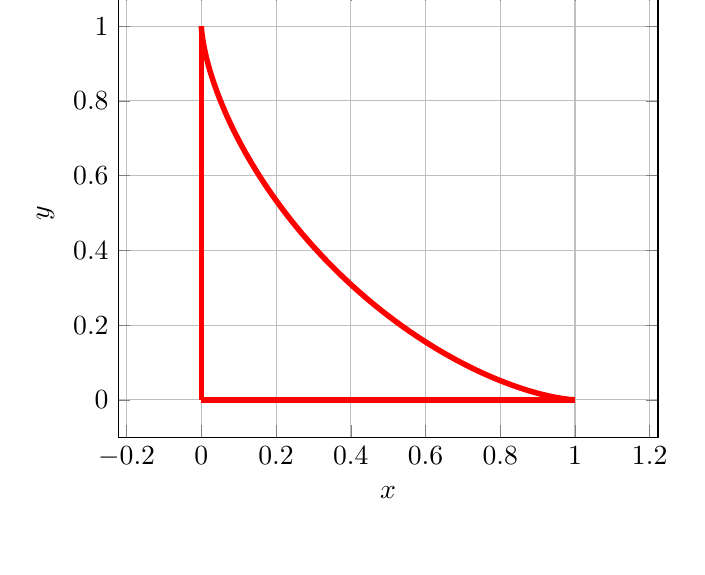
\begin{tikzpicture}
        \begin{axis}[
            xlabel={$x$},
            ylabel={$y$},
            axis equal,
            grid=major,
            domain=0:1,
            samples=200,
        ]
        \addplot+[mark=none,color=red, line width=2pt] ({sin(deg(x*pi/2))^3}, {cos(deg(x*pi/2))^3});
        \addplot+[mark=none,color=red, line width=2pt] ({0}, {x});
        \addplot+[mark=none,color=red, line width=2pt] ({x}, {0});
        \end{axis}
    \end{tikzpicture}
    \end{center}
    The curved part of the curve can be parameterized by 
    \begin{align*}
        \gamma : \left[0,\frac{\pi}{2}\right] \to \bbR^2, \quad t \mapsto \left( \cos^3(t), \sin^3(t) \right).
    \end{align*}
    \begin{itemize}
        \item Find parameterizations of the other two curves.
        \item With the $\vec F(x_1,x_2) = (x_2,-x_1)$ compute the curve integral 
        \[ \oint_C \vec F dl \]
        \item Use Green's theorem to explain how to compute the size of the area enclosed by the curve $C$.
    \end{itemize}
\end{exercise}
\begin{solution}     
\begin{itemize}
\item\begin{align*}
        \gamma_1 : \left[0,1\right] \to \bbR^2, \quad t \mapsto \left( 0, -t \right).
    \end{align*}
\begin{align*}
        \gamma_2 : \left[0,1\right] \to \bbR^2, \quad t \mapsto \left( t, 0 \right).
    \end{align*}
\item \begin{align*}
\oint_C \vec F dl &= \int_0^1 \begin{pmatrix} -t\\ 0\end{pmatrix}\cdot \begin{pmatrix} 0\\ -1\end{pmatrix}dt +  \int_0^1 \begin{pmatrix} 0\\ -t\end{pmatrix}\cdot \begin{pmatrix} 1\\ 0\end{pmatrix}dt +  \int_0^{\frac{\pi}{2}} \begin{pmatrix} \sin^3t\\ -\cos^3 t\end{pmatrix}\cdot \begin{pmatrix} -3\cos^2 t \sin t\\ 3\sin^2 t \cos t\end{pmatrix}dt\\
=&\int_0^{\frac{\pi}{2}} -3\cos^2 t\sin^2 tdt\\
=&\int_0^{\frac{\pi}{2}} -\frac{3}{4}\sin^2 2t dt\\
=&\int_0^{\frac{\pi}{2}} \frac{3}{4}\left(\frac{1}{2} \cos 4t - \frac{1}{2}\right)dt\\
=&\int_0^{\frac{\pi}{2}} -\frac{3}{8}dt = -\frac{3\pi}{16}
\end{align*}
\item We want to evaluate:
$$
\iint_{\Omega} 1 dxdy
$$

and Green's theorem tells us that:

$$
\oint_C \vec F dl  = \iint_{\Omega} \frac{\partial F_2}{\partial x_1} - \frac{\partial F_1}{\partial x_2} dx_1dx_2
$$

In the previous exercise we solved the line integral with the vector field $\vec F(x_1,x_2) = (x_2,-x_1)$. If we apply Greens theorem for this vector field then

$$
-\frac{3\pi}{16} = \oint_C \vec F dl  =  \iint_{\Omega} \frac{\partial F_2}{\partial x_1} - \frac{\partial F_1}{\partial x_2} dx_1dx_2 = \iint_{\Omega} -2 dx_1dx_2
$$

Therefore we have that

$$
-\frac{3\pi}{16} =  \iint_{\Omega} -2 dx_1dx_2
$$

and consequently 

$$
\frac{3\pi}{32} =  \iint_{\Omega} dx_1dx_2
$$
\end{itemize}
\end{solution}


\begin{exercise}[Stokes's theorem]
    We have a vector field 
    \begin{align*}
        \vec F( x_1, x_2, x_3 ) = \left( x_1 x_2, x_2 x_3, x_1 x_3 \right)
    \end{align*}
    and a surface 
    \begin{align*}
        S := \left\{ (x_1,x_2,x_3) \in \bbR^{3} \suchthat* x_1^2 + x_2^2 + x_3^2 = 1, \; x_2 \geq 0, x_3 \geq 0 \right\} 
    \end{align*}
    \begin{itemize}
        \item Find parameterizations of the surface $S$ and a parameterization of its boundary curve $C$.
        \item Use Stokes' theorem to compute the integral 
        \begin{align*}
            \iint_{S} \operatorname{curl} \vec F \;d\sigma.
        \end{align*}
    \end{itemize}
\end{exercise}
\begin{solution}     
The surface is parameterized by $$\Omega := [0,\pi]\times[0,\frac{\pi}{2}] \mapsto S: (\theta, \phi) \mapsto (\cos\theta\sin\phi, \sin\theta\sin\phi, \cos\phi)$$
The boundary of domain $S$ is parameterised by two curves
\begin{align*}
        &\gamma_1 : \left[0,\pi\right] \to \bbR^3, \quad t \mapsto (\cos t, \sin t, 0),\\
        &\gamma_2 : \left[
0,\pi\right] \to \bbR^3, \quad t \mapsto (-\cos t, 0, \sin t),\\
\end{align*}

Note that we do not need $\Phi\circ\gamma_3$ to parameterise the boundary of $S$. Moreover it is not a regular parameterisation.

 \begin{align*}
         \iint_{S} \operatorname{curl} \vec F \;d\sigma &=  \int_0^{\pi} \begin{pmatrix} \cos t \sin t\\ 0 \\ 0\end{pmatrix}\cdot \begin{pmatrix} -\sin t\\ \cos t \\ 0\end{pmatrix}dt +  \int_0^{\pi} \begin{pmatrix} 0\\ 0 \\ -\sin t \cos t\end{pmatrix}\cdot \begin{pmatrix} \sin t\\ 0 \\ \cos t\end{pmatrix}dt\\ 
=& \int_0^{\pi} -\cos t \sin^2 t dt - \int_0^{\pi} \sin t \cos^2 t dt\\
=& -\int_0^0 u^2 du - \int_{-1}^1 v^2 dv\\
=& -\frac{2}{3}
\end{align*}
\end{solution}

% 
% 
% 
% \begin{exercise}
%     \textit{This is for fun and entertainment only.}
%     Compute 
%     \[
%         \sqrt{ 500 \cdot 501 \cdot 502 \cdot 503 + 1 }
%     \]
%     without using a calculator.
% \end{exercise}
% \begin{solution}
%     Inside the square root, we find 
%     \begin{align*}
%         &
%         500 \cdot 501 \cdot 502 \cdot 503 + 1
%         \\&=
%         500 \cdot (500+1) \cdot (500+2) \cdot (500+3) + 1
%         \\&=
%         500^4 + 6 \cdot 500^3 + ( 2 + 3 + 6 ) \cdot 500^2 + 6 \cdot 500 + 1
%         \\&=
%         500^4 + 6 \cdot 500^3 + 11 \cdot 500^2 + 6 \cdot 500 + 1
%         .
%     \end{align*}
%     A sharp look reveals that this equals 
%     \begin{align*}
%         &
%         500^4 + 6 \cdot 500^3 + 11 \cdot 500^2 + 6 \cdot 500 + 1
%         =
%         ( 500^2 + 3 \cdot 500 + 1 )^2
%         .
%     \end{align*}
%     Therefore,
%     \[
%         \sqrt{ 500 \cdot 501 \cdot 502 \cdot 503 + 1 } = 500^2 + 3 \cdot 500 + 1 = 250000 + 1500 + 1
%     \]
%     The total result is $251501$. Which happens to be a prime number.
% \end{solution}

\end{document}
